\documentclass[11pt]{article}
\usepackage[utf8]{inputenc}
\usepackage{amsmath}
\usepackage{amsfonts}
\usepackage{amssymb}
\usepackage{tikz}
\usepackage{pgfplots}
\pgfplotsset{compat=1.15}
\begin{document}
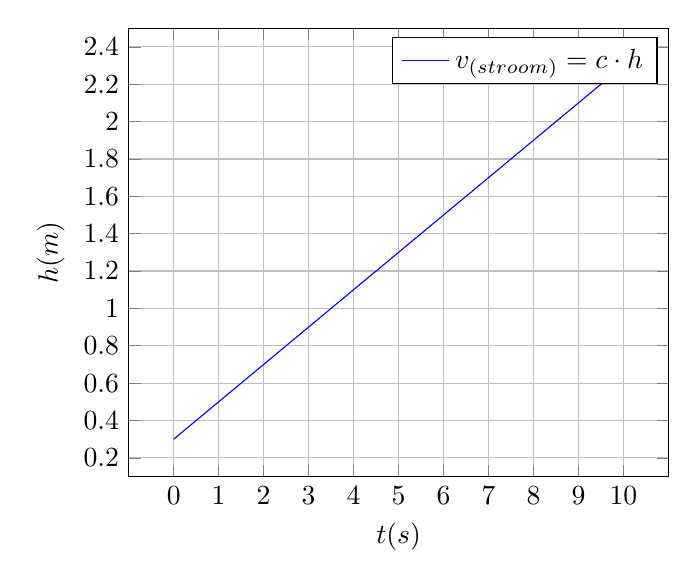
\begin{tikzpicture}
\begin{axis}[
%    axis lines=left
    xlabel=$t(s)$,
    ylabel=$h(m)$,
 	grid=both,
 	xtick={0,1,2,3,4,5,6,7,8,9,10},
 	ytick={0,0.2,0.4,0.6,0.8,1.0,1.2,1.4,1.6,1.8,2.0,2.2,2.4,2.6},
]
\addplot[
    domain=0:10,
    samples=100,
    color=blue,
]
{0.20*x+0.3};
\addlegendentry{$v_{(stroom)} = c \cdot h$}
%\addplot[
%color=blue,
 %   mark=square,
  %  ]
  %  coordinates {
   % (0,0.3)(0.10,0.32)(0.20,0.34)(0.30,0.36)(0.40,0.38)(0.50,0.40)(0.60,0.42)(0.70,0.44)
    %};
    %]
\end{axis}
\end{tikzpicture}

\end{document}